
\documentclass[conference]{IEEEtran}
\usepackage{url}
\usepackage{graphicx}
\usepackage{array}

\begin{document}


\title{Electronic Patient Consent Management}

\author{\IEEEauthorblockN{Atif Khan, Sarah Nadi}
\IEEEauthorblockA{David R. Cheriton School of Computer Science\\
University of Waterloo\\
Ontario, Canada\\
{{a78khan, snadi}@uwaterloo.ca}}
}

% make the title area
\maketitle


\begin{abstract}
Managing patients' information is very important for proper health care. As Information Communication Technologies (ICT) is being integrated into the medical
domain, patients' information is becoming increasingly managed through electronic systems. This poses the problem of managing patients' privacy
electronically according to each patient's consent policy. Accordingly, there is a need for an electronic patient consent management
system which captures patients' consent, and is able to process it and decide who can access the patient's information accordingly. In this paper, we propose
such a system where patient information and consent policies as well as other access policies are represented in Notation 3 (N3). A reasoning engine,
Euler, is used to determine if access should be granted or denied according to the patient's consent policy. We built a prototype to show the applicability of
using an RDF notation, such as N3, and Euler. We currently support five different consent policies: opt in, opt in with exceptions to specific people, opt in
with exceptions to sensitive information, opt out, and opt out with emergency override. In our prototype, we demonstrate how these consent policies affect
information access in different patient situations through twelve different scenarios.
\end{abstract}



\section{Introduction}
With the advance of Information Communication Technologies (ICT), more medical organizations are utilizing electronic systems to capture, manage and use patient
related information.  The scope of this information varies from organization wide Electronic Medical Records (EMRs) to Electronic Health Records (EHRs) shared
between different organizations.  Although this improves the effectiveness of information exchange, coordination, and use, it also raises the critical issue of
patient privacy. Usually, patient information is collected for the primary purpose of providing health care for a specific episode. Any secondary use must be in
accordance with patient consent.  It has been argued that a patient should be aware of all the systems collecting their information, and should be able to
specify how this information can be used~\cite{kluge2004informed}. Accordingly, each patient should choose a consent policy that reflects how they would like
their medical information to be used. Ideally, in an electronic system, the system would automatically grant or deny permission to
accessing a patient's record according to their specific consent policy. However, it is often difficult, if not impossible, to predict all future-use scenarios
and enforce patient consent in an appropriate manner. It should be noted that in this context, patient consent is related to accessing medical information.
This is different from the patient consent needed to provide certain treatment or perform a specific procedure, for example.

There are many aspects of this problem that need to be solved. First, how can patient consent be effectively and accurately captured electronically?
Second, how can the captured consent policies be represented and processed internally? Finally, how can we define consent policies that protect the patient
privacy, but do not compromise their health at the same time? All three problems are very important in this domain. However, in this paper, we focus on the
second problem, and
briefly touch upon the third.


To address these problems, we propose building a policy based (rule based) patient consent management system. The system would utilize (previously captured)
patient consent
information and various operational policies as input. Each policy will be represented by a set of RDF rules in Notation 3 (N3)~\cite{N3not}.  We will use the
Euler proof mechanism~\cite{eurlorprf} to compute (a) the result and (b) the proof of the aggregated rules.  


Our goal is to demonstrate that access to patient information can be protected in a real-time manner by utilizing policy based consent management.
The advantage of using Euler to generate a proof is that in the future, proofs can be validated between different systems when exchanging EHRs. This offers a
major improvement over the current industry practice of patient consent management and secondary use of patient information. This paper describes the
preliminary effort in this direction where we apply our idea to a selection of consent policies and situations, and produce a working prototype.


The contributions of this work are as follows: 

\begin{itemize}
    \item A set of consent policies represented in N3 notation. These are expressed as N3 rules which allow or deny access to the specified documents.

\item A collection of executable scenarios that show how the consent policies are applied in different situations.
\item A working prototype, implemented in Java, to demonstrate these scenarios.
\end{itemize}

The rest of this paper is organized as follows. Section~\ref{bg-sec} provides background information about patient consent, N3 notation, and the Euler engine.
Section~\ref{rel-work} describes some of the related work that has been done to develop an electronic patient consent system. Section~\ref{cons-polic} explains
the different consent policies, and specifies those included in our prototype. Section~\ref{main-sys} describes the prototype system developed in this
work. It describes the information flow in the system as well as the policy rules and facts used. Section~\ref{sec:discFuture} mentions some of the
limitations of our system and the possible future work we can do to address them. Finally, Section~\ref{concl} concludes this paper.


\section{Background}
\label{bg-sec}

\subsection{Patient Consent}
\label{pat-consent}

\subsubsection*{The Consent Challenge}
Effective patient management involves collaboration between multiple parties, each making its contribution to the overall health care provided to the patient. 
An effective health care framework will not only support multiple (diverse) participants, but it will also ensure proper information exchange between these
participants to ensure the highest level of service (care).  Although the prevalent exchange of patient information drastically improves the care provided, it
does raise a major challenge of information management.  More specifically patients would like to maintain control over the various attributes of their private
and confidential personal information.  The attributes being access, collaboration, and revocation.  We refer to this as the “Consent Challenge” in the medical
arena.  It is important to note that the consent challenges are applicable to all patient information in all types of formats.  

\begin{table*}[!t]
\centering
 \begin{tabular}{m{1cm}|m{9cm}}
\textbf{Tool} & \textbf{Description}\\
\hline\hline
cwm & Developed by the Tim Berners-Lee~\cite{berners-lee2008}, cwm is a forward chain reasoner written in python for N3 and N3Logic.  It can be used for
querying, checking, transforming and filtering information.  Furthermore, cwm is able to reason using a first order logic but without classical negation.\\
\hline
Euler & Euler is an inference engine that supports logic based proofs .  It differs from cwm as it is a backward-chaining reasoner enhanced with Euler path
detection mechanism~\cite{naudts2003inference}.\\
\hline
Pychinko & Pychinko is an efficient Python implementation of the classic Rete pattern matching algorithm.  It utilizes an optimized implementation of the
algorithm to handle facts, expressed as triples, and process them using a set of N3 rules~\cite{berners-lee2008}.\\
 \end{tabular}
\label{tab:n3tools}
\caption{RDF/N3 Reasoning Tools}
\end{table*}

Provided that the modern health information systems deal with patient data in electronic format, the consent challenge mutates into an electronic consent
challenge.  Patient consent has to be integrated at an application native level in order for it to be useful. OKeefe et al.~\cite{okeefe2002implementation}
coin the term of eConsent and list the following as key attributes of an electronic patient consent management system:

\begin{itemize}
 \item There is no single “right” solution to the eConsent challenge as an eConsent system needs to be tailored for the needs of different environments. For
example, the degree to which eConsent plays the role of a gatekeeper, active audit or passive record should be customizable. 
\item The introduction of an eConsent system will formalize and potentially affect existing trust relationships between consumers and providers. 
\item A simple yet flexible model for eConsent, supported by education and training, is key to the acceptance and adoption of eConsent. 
\item A good set of default policies is key to ensuring that eConsent has a minimal impact on clinical workflow. For example, default policies for GP Clinics,
Mental Health Clinics, Sexual Health Clinics and Hospitals could be established. 
\item The manner in which eConsent is integrated with existing systems can significantly affect its effectiveness. 
\end{itemize}

\subsubsection*{The Semantic Challenge}
Although the above mentioned features promise a solid foundation, they lack some of the practical considerations that might arise from a multi-vendor,
multi-party health care information management infrastructure such as ours in Canada.  When different parties and their corresponding health information systems
are required to collaborate, the information exchange mechanism may not be optimal and may require a lowest common denominator approach to information
exchange. The major hurdle is not in the syntactic side, but rather in the semantic interoperability of information exchange.  This impedance mismatch (between
different vendor
systems) poses one of the major challenges to universal patient consent management. To apply the governing rules of patient consent, one must have a sound
semantic understanding of the consent as well as the data.  We term this as the “Semantic Challenge”.  

The semantic web technologies offer some primitive building blocks upon which a foundation for semantic consent management system could be laid on.  The
traditional information exchange protocols utilize a static predefined schema in order to define the data structure of the shared information. All exchanged
information is then governed (described) using the static schema.  The semantic web offers a different approach to solve the information exchange problem
between two dissimilar parties.  Each dataset is accompanied by a corresponding vocabulary.  Each vocabulary is described in a predefined and well understood
format, therefore making it possible to describe data in ways that make its semantics explicit and hence discoverable automatically in software.

“RDF is a standard model for data interchange on the Web. RDF has features that facilitate data merging even if the underlying schemas differ, and it
specifically supports the evolution of schemas over time without requiring all the data consumers to be changed~\cite{rdfsite}”.  These properties of RDF make
it an ideal candidate for management and exchange of medical information where the datasets (i) have a particular large set of consumers (ii)
enjoy a long life span and (iii) are constantly evolving.

\subsection{N3 Notation}

Notation 3 (N3) is based on RDF standards and represents an analogous syntax to RDF/XML to represent data.  Furthermore, N3 adds extra features like rules and
formulae in
order to process data and make inferences from facts in the data.  N3 is designed as an alternative to RDF's XML syntax with emphasis on (a) designed for a
human -readability and (b) scribblable language – easy to work with (less verbose compared to RDF/XML)~\cite{notation3}.  In N3, information is represented as a
set of statements, where each statement is composed of a subject, verb and an object. Each statement ends with a period.
For example an N3 statement:

\begin{table}[!h]
\centering
 \begin{tabular}{c}
 \textbf{{:thermo :temp :high}}.\\ 
 \end{tabular}
\end{table}


would translate into thermostat temperature is high. Similarly,

\begin{table}[!h]
\centering
 \begin{tabular}{c}
 \textbf{{:heating :power “0”}}.\\ 
 \end{tabular}
\end{table}

would translate into heating power is zero.  An N3 rule can be described by combining multiple N3 statements as such:

\begin{table}[!h]
\centering
\begin{tabular}{c}
\textbf{{:thermo :temp :high}. $=>$ {:heating :power “0”}.}\\
\end{tabular}
\end{table}


means that if the thermostat temperature is high, then the heating power is zero. As stated before, an N3 formula adds a considerable amount of deduction and
inference capabilities to a simple dataset.  “By having rules and data in the same
languages, N3 logic provides simplicity in syntax and completeness as rules can operate on themselves and anything written in N3 can be queried in N3
”~\cite{berners-lee2008}.


\subsection{Euler}

A reasoning engine is required in order to make use of the N3 rules.  There are various RDF/N3 reasoners available.
Table~\ref{tab:n3tools} highlights some of the most popular ones. We chose to use Euler because ???????????????


\section{Related Work}
\label{rel-work}

There are numerous studies dealing with electronic consent. However, these studies ignore the semantic aspect of information and focus
mainly on security aspects~\cite{reid2003, chen2009identity, blobel2004authorisation}. O'Keefe et al.~\cite{okeefe2002implementation} undertake a feasibility
study of electronic consent management system in medical arena. They expose various challenges faced by different consumer groups of electronic consent
management systems.  The study provides a sound set of recommendations for a generic implementation of a patient consent management system.
Song et al.~\cite{song2002patient} introduce the notion of an e-consent object, encompassing all relevant information concerning the patient consent in the
e-consent object. Lack of semantics is the biggest draw back of this model.  The rules of consent are not expressed in any formal language and therefore are
ambigious at interpretation time.
Win et al.~\cite{win2002implementing} describe an interface based approach through which patient consent can be expressed.  The solution lacks organic growth as
it hard codes the information and lacks the required flexibility for the user.
Pruski et al.~\cite{pruski2010} propose e-CRL language designed with the following two goals in mind (a) facilitate capturing of patient consent information (b)
formalize the expression of patient consent information.  ``The language has a well defined BNF based syntax and semantics defined based on first-order logic
and set theory which allow eHealth systems to fully control the access to critical health data.''  Although the e-CRL language provides support for semantics,
it lacks some important features such as proof generation.  Furthermore, the defined language is not compatible with the RDF based solutions and approaches
making integration difficult.


\section{Consent Policies}
\label{cons-polic}

\begin{table*}[!t]
\centering
\scalebox{0.75}{
 \begin{tabular}{m{3cm}|m{9cm}|m{5cm}}
\textbf{Query}&\textbf{Relevant Facts}&\textbf{Expected Results}\\
\hline\hline
Dr Smith $\rightarrow$ XRay1 & \begin{itemize}
                             \item Dr Smith is a member of Grand River 
\item Grand River has a by shift policy 
\item Dr Smith is on shift in Grand River
\item XRay1 belongs to John
\item John is treated in Grand River 
\item Dr Smith treats John 
\item John has an opt in policy 
                            \end{itemize} & Dr Smith is granted access\\
\hline
Dr Smith $\rightarrow$ BloodTest & \begin{itemize}
                          \item Dr Smith is a member of St Mary's 
\item St Mary's has a by shift policy
\item BloodTest belongs to Tim
\item Tim is treated in St Mary's
\item Dr Smith treats Tim
\item Tim has an opt in policy
                         \end{itemize} & Dr Smith is denied access because St Mary's has a by shift policy and he is not currently on shift\\
\hline
Dr Smith $\rightarrow$ CTScan3 & \begin{itemize}
                        \item Dr Smith is a member of St Catherine's
\item St Catherine's has a members only policy
\item CTSCan3 belongs to Sally
\item Dr Smith treats Sally
\item Sally has an opt in policy
                       \end{itemize} & Dr Smith is granted access even though he is not on shift because St Catherin's does not have a by shift only policy\\
\hline
Dr Jane $\rightarrow$ BloodTest & \begin{itemize}
                           \item Dr Jane is a member of St Mary's
\item St Mary's has a members only policy
\item Dr Jane is on shift at St Mary's
\item BloodTest belongs to Tim
\item TIm is treated in St Mary's
\item Dr Smith treats Tim
\item Tim has an opt in policy
                          \end{itemize} & Dr Jane is denied access because she is not treating Tim\\
\hline
Dr Smith $\rightarrow$ CTScan1 & \begin{itemize}
                                  \item Dr Smith is a member of Grand River
\item Grand River has a by shift policy
\item Dr Smith is on shift in Grand River
\item CTScan1 belongs to Peter
\item Peter is treated in Grand River
\item Dr Smith treats Peter
\item Peter has an opt out policy
                                 \end{itemize} & Dr Smith is denied access because Peter has an opt out policy\\
\hline
Dr Jane $\rightarrow$ XRay2 & \begin{itemize}
                               \item Dr Jane is a member of St Mary's
\item St Mary's has a by shift policy
\item Dr Jane is on shift in St Mary's
\item XRay2 belongs to Wendy
\item Wendy is treated in St Mary's
\item Dr Jane treats Wendy
\item Wendy has an opt out with emergency override policy
\item Wendy is in an emergency situation
                              \end{itemize} & Dr Jane is granted access since Wendy is in an emergency\\
\hline
NurseAlex $\rightarrow$ XRay2 & \begin{itemize}
                               \item Nurse Alex is a member of St Mary's
\item St Mary's has a by shift policy
\item Nurse Alex is on shift in St Mary's
\item XRay2 belongs to Wendy
\item Wendy is treated in St Mary's
\item Wendy has an opt out policy with emergency override
\item Wendy is in an emergency situation
\end{itemize} & Nurse Alex is granted access even though she is not treating Wendy because Wendy is in an emergency\\
\hline
Dr Jane $\rightarrow$ XRay3 & \begin{itemize}
                               \item Dr Jane is a member of St Mary's
\item St Mary's has a by shift policy
\item Dr Jane is on shift in St Mary's
\item XRay3 belongs to Jenna
\item Dr Jane treats Jenna
\item Jenna has an opt out policy with emergency override \end{itemize} & Dr Jane is denied access because Jenna has an opt out policy with emergency override,
and Jenna is not in an emergency\\
\hline
Dr Smith $\rightarrow$ CTScan2 & \begin{itemize}
                                  \item Dr Smith is a member of Grand River
\item Grand River has a by shift policy
\item Dr Smith is on shift at Grand River
\item CTScan2 belongs to Tom
\item Tom is treated in Grand River
\item Dr Smith treats Tom
\item Tom has an opt in policy with the exception of sensitive documents
                                 \end{itemize} & Dr Smith is granted access because CTScan2 is not classified as sensitive\\
\hline
Dr Smith $\rightarrow$ HIVRep1 & \begin{itemize}
                                  \item Dr Smith is a member of Grand River
\item Grand River has a by shift policy
\item Dr Smith is on shift at Grand River
\item HIVRep1 belongs to Tom
\item Tom is treated in Grand River
\item Dr Smith treats Tom
\item Tom has an opt in policy with the exception of sensitive documents
\item HIVRep1 is classified as sensitive
                                 \end{itemize} & Dr Smith is denied access because Tom has denied access to sensitive documents, and HIVRep1 is classified as
sensitive\\
\hline
Dr Smith $\rightarrow$ STD1 & \begin{itemize}
                               \item Dr Smith is a member of Grand River
\item Grand River has a by shift policy
\item Dr Smith is on shift at Grand River
\item STD1 belongs to John
\item John is treated in Grand River
\item Dr Smith treats John
\item John has an opt in policy
\item STD1 is classified as sensitive
                              \end{itemize} & Dr Smith is granted access even though STD1 is sensitive because John has a full opt in policy\\

\hline
Dr Smith $\rightarrow$ MRI1 & \begin{itemize}
                               \item Dr Smith is a member of St Catherine's
\item St Catherine's has a members only policy
\item MRI1 belongs to Jack
\item Jack is treated in St Catherine's
\item Jack has an opt in policy with specific denials to certain people
\item Jack has denied access to Dr Smith
                              \end{itemize} & Dr Smith is denied access since Jack has explicitly denied him in his policy\\                           
\end{tabular}
}
\caption{Summary of the tested scenarios}
\label{tab:scenarios}
\end{table*}



There are different forms of consent that a patient may choose from. Coiera and Clarke~\cite{coiera2004consent} define four general forms of patient consent as
follows:

\begin{itemize}
 \item \textit{General consent}: This is also generally known as ``opt-in'' which means that the patient agrees that any health care professional may access
all of their health data for the purpose of providing care to them.
\item \textit{General consent with specific denial(s)}: This means that the patient specifically defines certain exceptions to their general consent policy.
These exceptions may be related to particular data or to particular people.
\item \textit{General denial with specific consent(s)}: In this case, the patient generally denies access to their data except in specific circumstances. These
may include disclosure for specific purposes or to specific people or the disclosure of certain types of information.
\item \textit{General denial}: This is the strictest level of consent a patient may have. In this case, the patient denies the use of their information for any
future event irrelevant of the circumstances that may occur. This consent policy is also generally known as ``opt-out''.
\end{itemize}

Pruski~\cite{pruski2010} use these four forms of consent while designing their rule-based language for describing patient consent policies. Additionally,
Pruski outlines the key requirements that must be taken into consideration while dealing with patient consent. These are expressing who can access the data,
the kind and the sensitivity of the data, the period for which a consent policy is valid, the purpose of why the data is being accessed, and what kind of
consent is given to the user requesting the data. 

In our work, we consider both the four forms of patient consent as well as some of the requirements proposed by Pruski. In our current prototype, we support
five types of patient consent policies as follows:

\begin{itemize}
 \item \textit{opt-in}: As described above, a patient who has an opt-in policy allows any treating doctor to access their information. In our system, we also
add other conditions that need to be met such as that the health care professional should be a member of the admitting organization etc. These details will be
discussed in Section~\ref{main-sys}.
\item \textit{opt-in except for sensitive documents}: In this case, the patient allows access to all their information except for documents that are classified
as sensitive. For example, these may include HIV tests or Sexually Transmitted Diseases. 
\item \textit{opt-in except for certain people}: In this case, the patient allows access to all their information, but specifically denies certain individuals
from accessing their data. We currently support exceptions to health care professionals only.
\item \textit{opt-out}: A patient with an opt-out policy explicitly denies access to all their information regardless of who is trying to access the data or
why they are trying to access it.
\item \textit{opt-out with emergency override}: In this case, the patient agrees to grant access to their information only if it is an emergency situation. 
\end{itemize}

\begin{figure}[!t]
 \centering
 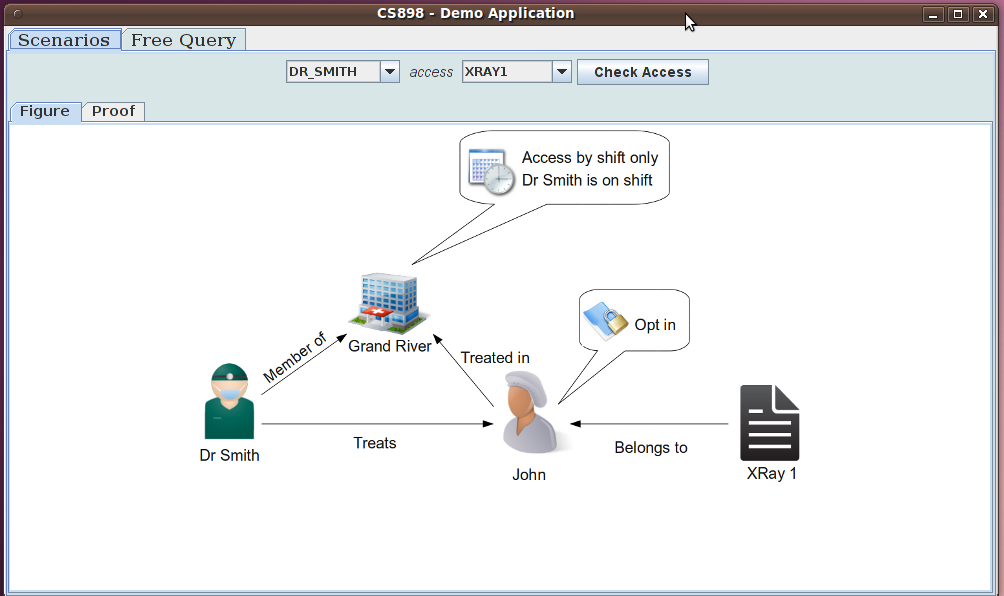
\includegraphics[scale=0.25,keepaspectratio=true]{./main.png}
 % main.png: 1004x596 pixel, 72dpi, 35.41x21.02 cm, bb=0 0 1004 596
 \caption{Example Scenario}
 \label{fig:mainscreen}
\end{figure}


\section{Our System Name}
\label{main-sys}

Not sure of this section's title but if we have a name for our system, that would do for the title. 

\subsection{Information Flow}
\label{info-flow}

Currently, our system assumes that all the information needed is already captured. That is, all information about the patient, their documents as well as their
privacy policies. Similarly, we also assume that all the information about the different hospitals, doctors, and nurses is already present. In this sense, we
focus on answering the question of whether a doctor or nurse can access a certain document. This is done by loading the facts available and our rule set into
Euler, and then querying it to see if a certain doctor or nurse can access a certain document. If access is granted, then we present the user with the proof
provided by Euler. If no proof is found, we check if we can find an explicit deny rule for the same actor and document in the original query. If so, we present
the user with the proof of why access has been denied. Figure~\ref{fig:mainscreen} shows the setup of our tool. In this scenario, we are checking if Dr Smith
has access to XRay1. In the ``Figure'' tab, a visual representation of all the facts related to this scenario is presented. These facts are extracted form
the facts.n3 file described in the next section. Once the user clicks on
``Check Access'', our tool would display Euler's generated proof as shown in Figure~\ref{fig:proof}. In this case, access has been granted as shown by the note
in
the top right corner. The proof shows the evidence used to reach this conclusion. It shows the different facts that have been used to satisfy the appropriate
rule to either grant or deny access.



\subsection{Facts in N3 Notation}

To test our access policies, we chose a set of facts that can reflect all the situations we wish to test. Figure~\ref{fig:allfacts} shows all the facts we use
to test our rules. There are four different types of actors: doctors, nurses, hospitals and patients. All hospitals have a ``members only'' policy where only
members of the hospital are authorized to access patient information. Some hospitals enforce a ``on shift'' only policy where only members that are currently on
shift may be able to access any patient information. Doctors and nurses can be members of more than one hospital, but can only be on shift in one hospital at a
time. A patient is treated in a hospital, and own documents that reflect their medical information. Some documents are classified as sensitive. Currently, we
only classify documents as sensitive or non sensitive (the default). In the future, we may wish to add different types of classifications such that a patient
may have more flexibility in specifying which category of documents do they grant access to. Additionally, a patient may be in an emergency situation. The
default is that the patient is in a regular episode of care. As indicated in Section~\ref{cons-polic}, we currently support five different types of patient
consent policies. These are coded as optin, optinsens, optinexcep, and optout respectively. We assigned the different policies to the patients such that all of
our designed access policies can be exhaustively tested. 
Appendix~\ref{sec:facts-file} shows the facts.n3 file we use to represent the facts shown in Figure~\ref{fig:allfacts}.

\begin{figure}[!t]
 \centering
 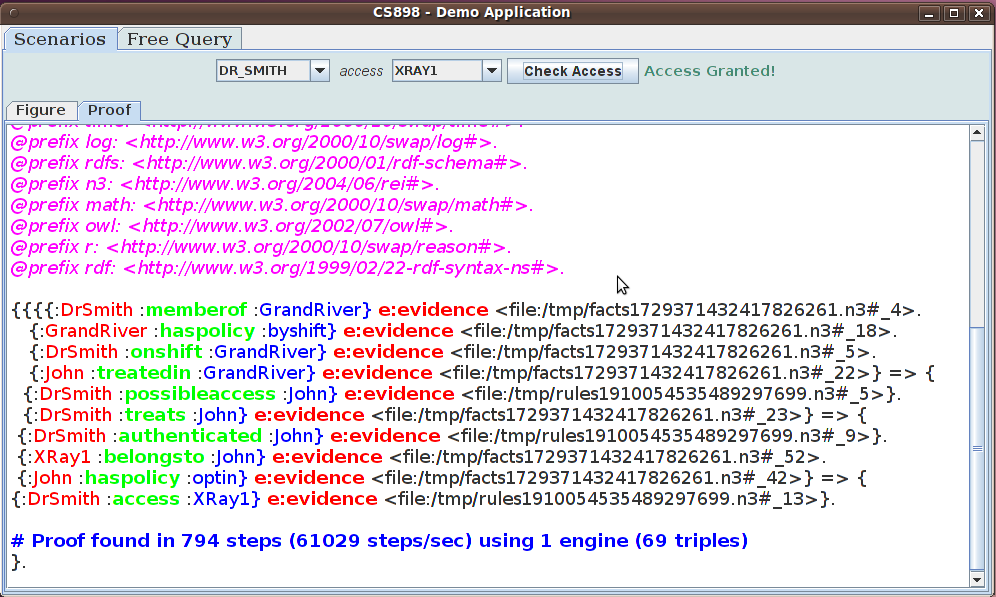
\includegraphics[scale=0.25,keepaspectratio=true]{./proof.png}
 % proof.png: 996x597 pixel, 72dpi, 35.13x21.06 cm, bb=0 0 996 597
 \caption{Query Result \& Proof of the Scenario in Figure~\ref{fig:mainscreen}}
 \label{fig:proof}
\end{figure}

\subsection{Access Policies in N3 Notation}
\label{rules-sec}

\begin{figure*}[t]
\centering
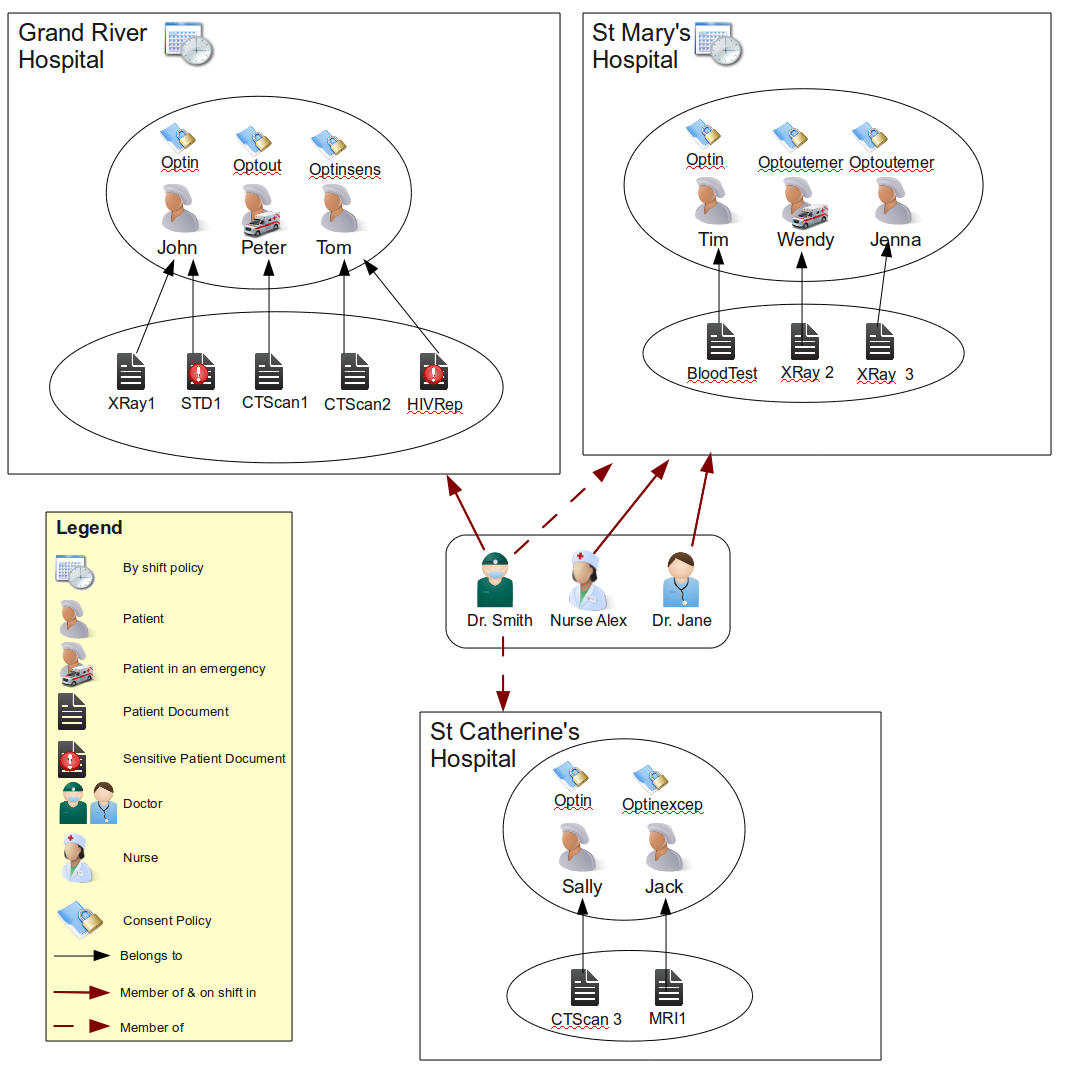
\includegraphics[width=16cm,height=14cm]{BigPicture.png}
\caption{Visual Representation of the facts.n3 File}
\label{fig:allfacts}
\end{figure*}

In our current prototype, we have designed the basic set of rules that can later be expanded for more sophisticated rule nesting. The complete rule file can be
found in Appendix~\ref{sec:rules-file}. There are six possible rule conclusions in our rule set. The two main conclusions are allowing or denying
access. However, we need the other rules to reach these conclusions. The following is the list of these six conclusions:



\begin{itemize}
 \item \textbf{\textit{possibleaccess}}: A person $a$ has possible access to patient $p$ if they are a member of the organization $p$ is treated in.
Additionally, if this organization has a by shift policy, then $a$ must be on shift to have possible access.
\item \textbf{\textit{authenticated}}: A person $a$ is authenticated to access a patient $p$'s information if they have possible access to $p$, and they are
treating $p$. The reason possible access is separated from authentication is that in emergency situations, a non treating doctor might need to access this
patient's information. In that case, they still need to satisfy the possible access rule.
\item \textbf{\textit{access}}: A person $a$ is granted access to a document $d$ if one of the following cases is true:
\begin{itemize}
 \item $a$ is authenticated to access $p$'s information, $d$ belongs to $p$, and $p$ has an opt in policy.
\item $a$ has possible access to $p$'s information, $d$ belongs to $p$, $p$ has an opt out policy with emergency override, and $p$ is in an emergency situation.
\item $a$ is authenticated to access $p$'s information, $d$ belongs to $p$, $p$ has an opt in policy with exceptions, and $a$ is not one of those exceptions.
\item $a$ is authenticated to access $p$'s information, $d$ belongs to $p$, $p$ has an opt in policy except for sensitive data, and $d$ is not classified as
sensitive.
\end{itemize}
\item \textbf{\textit{cannotaccess}}: This is the converse of the ``possibleaccess'' rule. A person $a$ does not have possible access $p$'s information if $p$
is treated in $o$, but $a$ is not a member of $o$. Similarly, if they are a member, but are not on shift in an organization that has a by shift policy, then $a$
does not have possible access to $p$'s information as well.
\item \textbf{\textit{notauthenticated}}: This is the opposite of the ``authenticated'' rule. If a person $a$ has possible access $p$'s information, but
$a$
does not treat $p$, then $a$ is not authenticated to access $p$'s information. If $a$ cannot access $p$'s information in the first place according to the
previous rule, then $a$ is automatically not authenticated to access $p$'s information.
\item \textbf{\textit{deny}}: A person $a$ is denied access to a document $d$ in one of the following situations:
\begin{itemize}
 \item $a$ is authenticated to access $p$'s information, $d$ belongs to $p$, but $p$ has an opt out policy.
\item $d$ belongs to $p$, but $a$ is not authenticated to access $p$'s information.
\item $a$ has possible access to $p$, $d$ belongs to $p$, $p$ has an opt out policy with emergency override, and the situation is not an emergency.
\item $a$ is authenticated to access $p$'s information, $d$ belongs to $p$, $p$ has an opt in policy except for sensitive information, and $d$ is classified as
sensitive.
\item $a$ is authenticated to access $p$'s information, $d$ belongs to $p$, $p$ has an opt in policy with specific denials, and $p$ has explicitly denied $a$
access.
\end{itemize}

\end{itemize}



\subsection{Tested Scenarios}

Given the above facts, we designed twelve different scenarios to test our different access policies. Table~\ref{tab:scenarios} summarizes these scenarios and
their expected results. In this table, we use plain English to describe the query and facts instead of n3 notation for better illustration. These facts are
based on the facts.n3 file shown in Appendix~\ref{sec:facts-file}, and represented in Figure~\ref{fig:allfacts}. We write the queries in the form of ``some
person $\rightarrow$ some document'' which means that this person is trying to
access this document, and we are trying to determine whether we should grant them access or not. As shown in Table~\ref{tab:scenarios}, we chose scenarios that
show how the different consent policies behave in different situations. For example, Tom has an opt in policy with the exception of sensitive documents. When
Dr Smith tries to access a non-sensitive document, CTScan2, he was granted access. However, when he tries to access a sensitive document, STD1, he was denied
access. Similarly, we tested different combination of facts for the other policies to demonstrate how they produce different results in different situations.


\section{Discussion and Future Work}
\label{sec:discFuture}

Our current work is a simple prototype demonstrating the applicability of using ideas from the semantic web to the problem of reasoning with patient consent.
Our prototype shows that using a reasoning engine such as Euler successfully provides the needed results. However, there are still some limitations to our
solution. Some of them can be easily implemented as future work, and some of them are due to the nature of N3 notation, and the way Euler works. 

Currently, we can only answer queries which have one answer. For example, we cannot answer queries in the form of ``Who has access to a specific document?''
This is because
Euler returns the first answer it finds which satisfies the query. It does not look for all possible solutions. There may be ways to get around this which we
are not currently aware of. As future work, it may be nice to provide such a querying functionality in the system.

To be able to address all medical situations, our rule set must be expanded. In this prototype, we demonstrated the basic consent policies. However, there are
many variations that can be added. For example, allowing family members to ask for access. The basic rule construction would be the same, but we just need to
build a rule ontology that accounts for all the possible situations. This leads to mentioning the need for more sophisticated rule writing in N3. N3
notation supports rule nesting which would support more elaborate policies. So far, we have focused on trying the basic features of writing
rules in N3. The next step would be to expand the rule set to include more consent policies using rule nesting.

In our current prototype, we do not discover policy conflicts. This would be a very useful feature to add. First, it would allow us to discover any mistakes
made while creating the rules. It would also be useful to detect conflicts between different levels of policies. For example, a hospital may have specific
policies that allow access to patient information in a specific situation, while the province policies deny access. Detecting such conflicts and resolving them
is important to achieve a fully functional electronic consent system. We currently only support ``access'' or ``deny'' results. In order to be more
specific, we plan to support more granular access levels in the future. For example, read, write, modify, delete etc. Finally, instead of hard coding patient
facts in N3 notation, having the relevant facts be automatically converted into N3 from an actual hospital database system would be more practical.
That way, already existing information can be used and integrated within an electronic patient consent management system.

\section{Conclusion}
\label{concl}

In this paper, we presented an electronic patient consent management system prototype. Our prototype is based on N3 notation, and the Euler reasoning engine.
We demonstrated five different patient consent policies (opt in, opt in with exceptions to sensitive information, opt in with exceptions to certain people, opt
out, and opt out with emergency override), and presented different scenarios to show how they affect access control in each situation. We tested twelve
different scenarios which present different fact combinations to show how the different consent policies behave in different situations. Our prototype shows
that using a semantic reasoning engine such as Euler works well to address the challenges of patient information access. The advantage of Euler is that it can
semantically reason with the data, and additionally, can generate a proof showing the evidence it found to support its conclusions. Such a proof can later be
used as a verification token to be exchanged between different systems. We hope to expand this prototype by supporting more consent policies, and more
elaborate rule nesting in N3 to achieve better support for patient consent management.



% use section* for acknowledgement
\section*{Acknowledgment}


We would like to thank Dr. Helen Chen for her guidance through the development of this prototype.  





%\IEEEtriggeratref{8}
% references section
\bibliographystyle{IEEEtran}
\bibliography{references}


\appendices

\onecolumn

\section{Facts File}
\label{sec:facts-file}

@prefix : $<\#>$. \newline
\newline
\#Nurses and Doctors \newline
:DrSmith :memberof :GrandRiver.\newline
:DrSmith :onshift :GrandRiver.\newline
:DrSmith :memberof :StMarys.\newline
:DrSmith :memberof :StCatherines.\newline
\newline
:DrJane :memberof :StMarys.\newline
:DrJane :onshift :StMarys.\newline
\newline
:NurseMary :memberof :GrandRiver.\newline
:NurseAlex :memberof :StMarys.\newline
:NurseAlex :onshift :StMarys.\newline
\newline
\#Hospital policies\newline
:StMarys :haspolicy :byshift.\newline
:GrandRiver :haspolicy :byshift.\newline
:StCatherines :haspolicy :members.\newline
\newline
\#Patients\newline
:John :treatedin :GrandRiver.\newline
:DrSmith :treats :John.\newline
:NurseMary :treats :John.\newline
:Tim :treatedin :StMarys.\newline
:DrSmith :treats :Tim.\newline
:Peter :treatedin :GrandRiver.\newline
:DrSmith :treats :Peter.\newline
:NurseAlex :treats :John.\newline
:Wendy :treatedin :StMarys.\newline
:DrJane :treats :Wendy.\newline
:Tom :treatedin :GrandRiver.\newline
:DrSmith :treats :Tom.\newline
:Jenna :treatedin :StMarys.\newline
:DrJane :treats :Jenna.\newline
:Sally :treatedin :StCatherines.\newline
:DrSmith :treats :Sally.\newline
:Jack :treatedin :StCatherines.\newline
:DrSmith :treats :Jack.\newline
\newline
\#Patients' consent policies\newline
:John :haspolicy :optin.\newline
:Tim :haspolicy :optin.\newline
:Peter :haspolicy :optout.\newline
:Wendy :haspolicy :optoutemer.\newline
:Tom :haspolicy :optinsens.\newline
:Jenna :haspolicy :optoutemer.\newline
:Sally :haspolicy :optin.\newline
:Jack :haspolicy :optinexcep.\newline
\newline
\#Patients' documents\newline
:XRay1 :belongsto :John.\newline
:STD1 :belongsto :John.\newline
:BloodTest :belongsto :Tim.\newline
:CTScan1 :belongsto :Peter.\newline
:XRay2 :belongsto :Wendy.\newline
:CTScan2 :belongsto :Tom.\newline
:HIVRep1 :belongsto :Tom.\newline
:XRay3 :belongsto :Jenna.\newline
:CTScan3 :belongsto :Sally.\newline
:MRI1 :belongsto :Jack.\newline
\newline
\#Patients' Situations\newline
:Peter :hassituation :emergency.\newline
:Wendy :hassituation :emergency.\newline
\newline
\#Documents' sensitivity\newline
:STD1 :hasnature :sensitive.\newline
:HIVRep1 :hasnature :sensitive.\newline
 \newline
\#Denial of access to specific people\newline
:Jack :denyaccess :DrSmith.\newline

\section{Rules File}
\label{sec:rules-file}

\#These rules checks if a has possible access to patient p's records. a must be a member of the same organization that p is \newline
\#treated in. Depending on the organization policy, member may have to be on shift. \newline 
\newline
{?a :memberof ?o. ?o :haspolicy :byshift. ?a :onshift ?o. ?p :treatedin ?o.} $=>$ {?a :possibleaccess ?p}.\newline 
\newline
{?a :memberof ?o. ?o :haspolicy :members. ?p :treatedin ?o.}  $=>$ {?a :possibleaccess ?p}.\newline
\newline
\#If a has possible access to patient p's records, and a treats p then a is authenticated to access p's records \newline
\newline
{?a :possibleaccess ?p. ?a :treats ?p.}  $=>$ {?a :authenticated ?p}.\newline 
\newline
\#If a has possible access to d, and p has a full optin policy then a can access d \newline
\newline
{?a :authenticated ?p. ?d :belongsto ?p. ?p :haspolicy :optin. }  $=>$ {?a :access ?d}.\newline
\newline
\#If a has possible access to d, and p has a an optout policy with emergency override and situation s is an emergency \newline
\#situation, then a can access d even if the dr is not the treating doctor \newline
\newline
{?a :possibleaccess ?p. ?d :belongsto ?p. ?p :haspolicy :optoutemer. ?p :hassituation :emergency} = $=>$ {?a :access ?d}. \newline
\newline
\#If p has an optin policy with exceptions, d belongs to p, and a is not one of those exceptions, then a is granted access\newline
\#to d. \newline
\newline
{?a :authenticated ?p. ?d :belongsto ?p. ?p :haspolicy :optinexcep. $<$facts.n3$>$ log:notIncludes {?p :denyaccess ?a}}  $=>$ {?a :access ?d}. \newline
\newline
\#If a has possible access to d, p has a opt in policy except for sensitive data, and d is not sensitive, then a \newline
\#can access d \newline
\newline
{?a :authenticated ?p. ?d :belongsto ?p. ?p :haspolicy :optinsens. $<$facts.n3$>$ log:notIncludes {?d :hasnature :sensitive}}  $=>$ {?a :access ?d}. \newline
\newline
\#DENIAL RULES
\newline
\#No possible access if a is not a member of the same organization p is treated in \newline
\newline
{?p :treatedin ?o. $<$facts.n3$>$ log:notIncludes {?a :memberof ?o}}  $=>$ {?a :cannotaccess ?p}.
\newline
\#No possible access if a is not on shift in an organization that has a by shift policy \newline
\newline
{?p :treatedin ?o. ?a :memberof ?o. ?o :haspolicy :byshift. $<$facts.n3$>$ log:notIncludes {?a :onshift ?o}}  $=>$ {?a :cannotaccess ?p}.
\newline
\#Not authenticated if a has possible access but does not treat p \newline
\newline
{?a :possibleaccess ?p. $<$facts.n3$>$ log:notIncludes {?a :treats ?p}}  $=>$ {?a :notauthenticated ?p}.
\newline
\#If a has possible access to d, and p has a an optout policy with emergency override and situation s is NOT an emergency \newline
\#situation, then a is denied access.\newline
\newline
{?a :possibleaccess ?p. ?d :belongsto ?p. ?p :haspolicy :optoutemer. $<$facts.n3$>$ log:notIncludes{?p :hassituation :emergency}}  $=>$ {?a :deny ?d}. \newline
\newline
\#If p has an opt in policy with exceptions and explicitly denies a doctor then access to this document is denied \newline
\newline
{?a :authenticated ?p. ?d :belongsto ?p. ?p :haspolicy :optinexcep. ?p :denyaccess ?a}  $=>$ {?a :deny ?d}. \newline
\newline
\# If a is authenticated, and p has a full optout policy, and \#document d belongs to patient p then a is denied access \newline
\#to d  \newline
\newline
{?a :authenticated ?p. ?d :belongsto ?p. ?p :haspolicy :optout.}  $=>$ {?a :deny ?d}. \newline
\newline
\#Not authenticated if a cannot access p (even though a treats p (maybe not on shift)). \newline
\newline
{?a :cannotaccess ?p.}  $=>$ {?a :notauthenticated ?p}. \newline
\newline
\#If a is not authenticated to treat p, then access is denied \newline
\newline
{?a :notauthenticated ?p. ?d :belongsto ?p}  $=>$ {?a :deny ?d}. \newline
\newline
\#If a is authenticated, d belongs to p, p has a an optin \#except to sensitive data, and d is sensitive then a is denied \newline
\#access \newline
\newline
{?a :authenticated ?p. ?d :belongsto ?p. ?p :haspolicy :optinsens. ?d :hasnature :sensitive}  $=>$ {?a :deny ?d}. \newline



% that's all folks
\end{document}


